\chapter{Spectroscopy}
\section{Atomic spectroscopy}
\subsection{Selection rules}
\begin{thrm}[The Laporte selection rule]
The Laporte selection rule states that electric dipole transition that does not involve a change in parity is strictly forbidden, while those involving a change in parity may be allowed. In other words, the only transitions allowed are those involving a change in parity.
\end{thrm}
\begin{proof}
The transition probability between two states are given by the Einstein `B' coefficient which is given in \cref{einsteincoeff}, which is proportional to the modulus squaured of the \emph{transition dipole moment}
\begin{equation}
	\bvec{\mu}_{i\rightarrow f}=\lgl i | \uvec{\mu} |f\rgl
\end{equation}
\Cref{zerointegral} tells that the integrand must contain the tot. sym. irrep of the group the particle belongs to, which in this case is the full rotation group $R_3$. The inversion operation\footnote{Just because we can readily deduce the parity from the orbital angular momentum. In principle any other operation is fine, we just need to see whether the direct product is $[1,1,\dots,1]$} is diagnostic: if the integrand is antisymmetrical wrt. inversion the integral is necessarily zero. \textbf{Parity} is just the $g/u$ label, but represented numerically as $\pm1$. The parity of atmoic orbitals is $(-1)^l$, because the dipole moment operator has $u$ symmetry, the overall parity of the integrand is
\begin{equation}
	(-1)^{l_i}(-1)(-1)^{l_f}
\end{equation}
which shows the two orbitals must have \emph{opposite parity} for the integral to be plausibly non-zero.
\end{proof}
This allows us to deduce the selection rule for orbital angular momentum of an atom
\begin{thrm}[Selection rule for orbital angular momentum]
The selection rule is 
\begin{equation}
	\Delta l=\pm1
\end{equation}
\end{thrm}
\begin{proof}
	As the dipole moment operator transforms like a translation which is exactly like $l=1$ spherical harmonics, the representative of $\uvec{\mu}$ is $\Gamma^{(1)} $. The overall direct product for $\lgl i | \uvec{\mu}|f \rgl $ is 
	\begin{equation}
	\begin{aligned}
		&\Gamma^{(l_i)}\otimes\Gamma^{(1)}\otimes\Gamma^{(l_f)}\\
		=&\lf(\Gamma^{(l_i+1)}\oplus\Gamma^{(l_i)}\oplus\Gamma^{(l_i-1)} \rt)\otimes\Gamma^{(l_f)}
	\end{aligned}
	\end{equation}
	The requirement is for the integrand to \emph{contain} the tot. sym. irrep, so clearly $\Gamma^{(l_f)}$ must be one of the three terms in front. And $\Delta l=0$ is Laporte forbidden so we are left with the selection rule of $\Delta l=\pm1$.
\end{proof}
The selection rule for $m_l$ can be deduced as well:
\begin{thrm}[Selection rule for magnetic quantum number]
The selection rule is
\begin{equation}
	\Delta m_l=0,\pm1
\end{equation}
\end{thrm}
\begin{proof}
	 We now just need to look at the $\phi$ dependence only, which gives us the integral of the form
\begin{equation}
	\int^{2\pi}_0e^{-im_{li}\phi}(\hat{\mu}_j)e^{im_{lf}\phi}\dif \phi
\end{equation}
with $\uvec{\mu}=-e\bvec{r}$ is the electric dipole operator, which in spherical coordinates is
\begin{equation}
	-er
	\begin{pmatrix}
		\sin\theta\cos\phi\\
		\sin\theta\sin\phi\\
		\cos\phi
	\end{pmatrix}
\end{equation}
Now considering radiation that is plane-polarised with the electric field in the $z$-direction, remembering the first bra represents the complex conjugate, we get
\begin{equation}
	\int^{2\pi}_0e^{-im_{lf}\phi}(-er\cos\theta)e^{im_{li}\phi}\dif \phi\propto\int^{2\pi}_0e^{i(m_{li}-m_{lf})\phi}\dif \phi
\end{equation}
which gives $\Delta m_l=0$. If the radiation is polarised in the $x$-direction, we have
\begin{equation}
\begin{aligned}
	&\int^{2\pi}_0e^{-im_{li}\phi}(-er\sin\theta\cos\phi)e^{im_{lf}\phi}\dif \phi\\
	\propto&\int^{2\pi}_0e^{-im_{li}\phi}(e^{i\phi}+e^{-i\phi})e^{im_{lf}\phi}\dif \phi\\
	=&\int^{2\pi}_0e^{i(m_{lf}-m_{li}+1)\phi}+e^{i(m_{lf}-m_{li}-1)\phi}\dif \phi
\end{aligned}
\end{equation}
which means, to have a non-zero result, $\Delta m_l=\pm1$. The $y$-polarised radiation gives the same result.
\end{proof}
\subsection{Fine structure}
Spectroscopy measures transitions between energy levels, for example photoelectron spectroscopy measures that between electronic levels, and IR and Raman spectroscopy measures that between vibrational levels, and NMR between nuclear spin levels. By the same token, the energy differences between electronic spin levels can also be measured, and we'll develop some theoretical treatments to elucidate the fine structure of atomic spectra.
\subsubsection{Orbital and spin magnetic moments}
\paragraph{Orbital magnetic moment}
The orbital magentic moment can be derived from classical arguments: the current ($\diff qt$) of a circulating electron in the $xy$-plane at speed $v$ at radius $r$ is
\begin{equation}
 	I=-\frac{ev}{2\pi r}
\end{equation} 
The magnetic dipole in the $z$-direction is
\begin{equation}
	m_z=IA=-\frac{ev}{2\pi r}\times\pi r^2=-\tfrac{1}{2}evr
\end{equation}
The $z$-component of the angular momentum is 
\begin{equation}
	l_z=m_{\mathrm{e}}vr
\end{equation}
so
\begin{equation}
	m_z=\underbrace{-\frac{e}{2m_{\mathrm{e}}}}_{\gamma_{\mathrm{e}}} l_z
\end{equation}
As the argument holds in all three cardinal directions, we arrive at the simple relation
\begin{equation}
	\bvec{m}=\gamma_{\mathrm{e}}\bvec{l}
\end{equation}
where $\gamma_{\mathrm{e}}=-e/2m_{\mathrm{e}}$ is called the \emph{gyromagnetic ratio} of the electron.\par
Now we're done with the classical and technically incorrect derivation, we need to introduce the quantum mechanical quantisation by claiming $m_z$ is quantised like $l_z$, namely
\begin{equation}
	m_z=\gamma_{\mathrm{e}}m_l\hbar,\ \ m_l=-l,-l+1,\dots,l
\end{equation}
and we can define the \emph{Bohr magneton} as $\mu_{\mathrm{B}}=-\gamma_{\mathrm{e}}\hbar=e\hbar/2m_{\mathrm{e}}$ so we can write
\begin{equation}
	m_z=-\mu_{\mathrm{B}}m_l,\ \ |m_l|=0,1,\dots,l
\end{equation}
\paragraph{Spin magnetic moment}
The orbital angular momentum has a classical analogue whereas the intrinsic spin does not. We can't rely on classical arguments here because there are none. It turns out that for the spin magnetic moment, 
\begin{equation}
\begin{aligned}
	&\bvec{m}=g_{\mathrm{e}}\gamma_{\mathrm{e}}\bvec{s},\ \ g_{\mathrm{e}}\approx2\\
	&m_z=-g_{\mathrm{e}}\mu_{\mathrm{B}}m_s,\ \ m_s=\pm\tfrac{1}{2}
\end{aligned}
\end{equation}
$g_{\mathrm{e}}$ is known as the \emph{$g$-factor}
\footnote{This is twice the expected value from claisscal mechanics. The full derivation of the factor requires the relativistic Dirac equation and even then a much smaller (0.00232) correction requires quantum electrodynamics. One interesting way to think about this is that the quantum mechanical rotation operator will return $\text{Rot}(2\pi)|\chi\rgl=-|\chi\rgl$, which in essence says that \emph{a full rotation in quantum mechanics is $4\pi$ radian instead of $2\pi$}! So the velocity of rotation and so on are all doubled.}.
The nuclear spin magentic moment obeys the same rule:
\begin{equation}
\begin{aligned}
	&\bvec{m}=g_{\mathrm{I}}\gamma_{\mathrm{N}}\bvec{I}\\
	&m_z=g_{\mathrm{I}}\mu_{\mathrm{N}}m_I,\ \ m_s=-I,-I+1,\dots,I
\end{aligned}
\end{equation}
where $\mu_{\mathrm{N}}=e\hbar/2m_{\mathrm{p}}$ is the \emph{nuclear magneton}, and $g_{\mathrm{I}}$ is the nuclear magneton, of order $10^0$.
\paragraph{Land{\'e} $g$-factor}
For an electron with both orbital and spin magnetic moment, the resultant magnetic moment is given exactly\footnote{The only approximation being, $g_{\mathrm{e}}=2$ which goes into the `offset' constant in front.} as
\begin{equation}
	\bvec{m}=g_{\mathrm{J}}\gamma\bvec{J}
\end{equation}
where $g_{\mathrm{J}}$ is the \emph{Land{\'e} coefficient}, given by
\begin{equation}
	g_{\mathrm{J}}=\tfrac{3}{2}+\frac{S(S+1)-L(L+1)}{2J(J+1)}
\end{equation}
\subsubsection{Spin-orbit coupling}
The Hamiltonian of spin-orbit coupling \emph{in an isotropic electric field} can be derived exactly:
\begin{equation}
	H_{\mathrm{so}}=\xi(r)\bvec{l}\cdot\bvec{s}
\end{equation}
where $\xi>0$ and is proportional to the first derivative of the electric potential $\phi$:
\begin{equation}
	\xi(r)=-\frac{e}{2m_{\mathrm{e}}^2rc^2}\diff{\phi}{r}
\end{equation}
and the \emph{spin-orbit coupling constant} is given by the radial average of $\xi(r)$:
\begin{equation}
	hc\xi_{nl}=\lgl nlm_l|\xi(r) |nlm_l  \rgl\hbar^2
\end{equation}
Given the hydrogen-like Coulombic field $\phi=Ze/4\pi\ep_0r$, the full Hamiltonian is then given as
\begin{equation}
\label{sochamil}
H_{\mathrm{so}}=\frac{Ze^2}{8\pi\ep_0m_{\mathrm{e}}^2r^3c^2}\bvec{l}\cdot\bvec{s} 	
\end{equation} 
we can derive
\begin{equation}
\label{xinl}
	\xi_{nl}=\frac{\alpha^2RZ^4}{n^3l(l+\tfrac{1}{2})(l+1)}
\end{equation}
where $\alpha=e^2/4\pi\ep_0\hbar c$ is the \emph{fine-structure constant}. Note that it goes as $Z^4$, which means the coupling constant rapidly increases in heavier elements.\par
The \emph{Russell-Saunders coupling} scheme says about the energies
\begin{equation*}
\text{spin-spin coupling > orbit-orbit coupling > spin-orbit coupling}
\end{equation*}
We need to explain this carefully:
\begin{enumerate}
	\item \textbf{Spin-spin coupling} means how strongly the spin angular momenta of the electrons interact, this is manifested by the Fermi holes, and more precisely, the \emph{exchange interactions}. This splits a configuration into terms of different multiplicities. However this is rarely resolved on its own as the next level of branching, terms, are widely spaced and usually well resolved, as a consequence these energy levels don't get a name of their own.
	\item \textbf{Orbit-orbit coupling} means how strongly orbital angular momenta interact - electrons that move in the same direction meet less than those that move in opposite directions. This splits the terms with the same multiplicity into terms.
	\item \textbf{Spin-orbit coupling} was explained above. It splits terms into levels. However to fully explain Hund's third rule we need some further discussions, given below.
	\item In the presence of \textbf{external magnetic fields} the levels are further split into states with the lowest $M_J$ having the lowest energy.
\end{enumerate}
So we can draw a schematic diagram like this
\begin{center}
\begin{tikzpicture}
\node[draw,fill=orange!60!white,below,text width=2cm,font=\tiny] at (2.5,-5) {Split by spin-spin coupling\\\textbf{Hund's first rule}};
\draw[-{Stealth}, line width=1mm] (2.5,-4.75)--(2.5,-1.5);
\node[draw,fill=orange!60!white,below,text width=2cm,font=\tiny] at (5.5,-5) {Split by orbit-orbit coupling\\\textbf{Hund's second rule}};
\draw[-{Stealth}, line width=1mm] (5.5,-4.75)--(5.5,-3);
\node[draw,fill=orange!60!white,below,text width=2cm,font=\tiny] at (8.5,-5) {Split by spin-orbit coupling\\\textbf{Hund's third rule}};
\draw[-{Stealth}, line width=1mm] (8.5,-4.75)--(8.5,-3.5);
\node[draw,fill=orange!60!white,below,text width=2cm,font=\tiny] at (11.5,-5) {Split by external magnetic field only};
\draw[-{Stealth}, line width=1mm] (11.5,-4.9)--(11.5,-4);
\draw[thick] (0,0) node[left]{$d^3$}-- node[below,align=center,font=\scriptsize\scshape]{Electron\\configuration}++(2,0);

%doublet terms
\draw[dashed](2,0)--(3,2);
\draw[thick](3,2)--node[below,align=center,font=\scriptsize\scshape]{Doublet\\terms}++(2,0);
\draw[dashed](5,2)--(6,3.5);
\draw[dashed](5,2)--(6,2.5);
\draw[dashed](5,2)--(6,1.5);
\draw[dashed](5,2)--(6,1);
\draw[dashed](5,2)--(6,0.5);
\draw[dashed](5,2)--(6,0);
\draw[thick](6,3.5)--++(2,0) node[right,font=\scriptsize]{$^2D$};
\draw[thick](6,2.5)--++(2,0) node[right,font=\scriptsize]{$^2F$};
\draw[thick](6,1.5)--++(2,0) node[right,font=\scriptsize]{$^2D$};
\draw[thick](6,1)--++(2,0) node[right,font=\scriptsize]{$^2P$};
\draw[thick](6,0.5)--++(2,0) node[right,font=\scriptsize]{$^2H$};
\draw[thick](6,0)--++(2,0) node[right,font=\scriptsize]{$^2G$};

%quartet terms
\draw[dashed](2,0)--(3,-2);
\draw[thick](3,-2)--node[below,align=center,font=\scriptsize\scshape]{Quartet\\terms}++(2,0);
\draw[dashed](5,-2)--(6,-1);
\draw[dashed](5,-2)--(6,-3);
\draw[thick](6,-1)--++(2,0) node[right,font=\scriptsize]{$^4P$};
\draw[thick](6,-3)--node[above right,font=\scriptsize]{$^4F$}node[below,font=\scriptsize\scshape]{Terms}++(2,0);

%4F levels
\draw[dashed](8,-3)--++(1,0.75);
\draw[dashed](8,-3)--++(1,0.25);
\draw[dashed](8,-3)--++(1,-0.25);
\draw[dashed](8,-3)--++(1,-0.75);
\draw[thick](9,-2.25)--++(2,0) node[right,font=\scriptsize]{$^4F_{9/2}$};
\draw[thick](9,-2.75)--++(2,0) node[right,font=\scriptsize]{$^4F_{7/2}$};
\draw[thick](9,-3.25)--++(2,0) node[right,font=\scriptsize]{$^4F_{5/2}$};
\draw[thick](9,-3.75)--node[above right,font=\scriptsize]{$^4F_{3/2}$}node[below,font=\scriptsize\scshape]{Levels}++(2,0);

%4F3/2 states
\draw[dashed](11,-3.75)--++(1,0.15);
\draw[dashed](11,-3.75)--++(1,0.05);
\draw[dashed](11,-3.75)--++(1,-0.05);
\draw[dashed](11,-3.75)--++(1,-0.15);
\draw[thick](12,-3.6)--++(2,0) node[above right,font=\scriptsize]{$^4F_{3/2}^{3/2}$};
\draw[thick](12,-3.7)--++(2,0) ;
\draw[thick](12,-3.8)--++(2,0) node[right] at (14,-3.65){\vdots};
\draw[thick](12,-3.9)--node[below,font=\scriptsize\scshape]{States}++(2,0) node[below right,font=\scriptsize]{$^4F_{3/2}^{-3/2}$};
\end{tikzpicture}

\end{center}
We now need to work out the exact expression for the energy separation between levels. Under the regime of Russell-Saunders coupling, we can apply first-order perturbation theory (see \Cref{1stpert}) to get the energy correction:
\begin{equation}
	E_{\mathrm{so}}=\lgl ls;jm_j|H_{\mathrm{so}} |ls;jm_j \rgl=\lgl ls;jm_j|\xi(r)\bvec{l}\cdot\bvec{s} |ls;jm_j \rgl
\end{equation}
note that this is the \emph{coupled picture}, which just specifies the individual angular momenta $l$ and $s$ and the resultant angular momentum $j$ and its $z$-component $m_j$, of a single electron\footnote{Note we've been using small case $l,s,j$, which is because so far we're only talking about single-electron states $|nlm_l\rgl$.}, the same coupled picture, but applied to composite angular momenta, with $\bvec{l}$ first building up to $\bvec{L}$ and $\bvec{m}$ to $\bvec{M}$, then both combine to give $\bvec{J}$, is the scheme under Russell-Saunders coupling. This discussion treats one-electron\par
We then write
\begin{equation}
	\bvec{j}^2=|\bvec{l}+\bvec{s}|^2=\bvec{l}^2+\bvec{s}^2+2\bvec{l}\cdot\bvec{s}
\end{equation}
so that
\begin{equation}
\begin{aligned}
\bvec{l}\cdot\bvec{s} |ls;jm_j \rgl&=\tfrac{1}{2}(\bvec{j}^2-\bvec{l}^2-\bvec{s}^2)|ls;jm_j \rgl\\
&=\tfrac{1}{2}\{j(j+1)-l(l+1)-s(s+1) \}|ls;jm_j \rgl
\end{aligned}
\end{equation}
where the boldface $\{\bvec{l},\bvec{j},\bvec{s}\}$ are operators and the the regular $\{l,j,s\}$ are the eigenvalues. We can write out the energy easily now, with reference to \cref{xinl},
\begin{equation}
\label{esoc}
\begin{aligned}
E_{\mathrm{so}}=&\tfrac{1}{2}\hbar^2\{j(j+1)-l(l+1)-s(s+1) \}\lgl ls;jm_j|\xi(r) |ls;jm_j  \rgl\\
=&\tfrac{1}{2}hc\xi_{nl}\{j(j+1)-l(l+1)-s(s+1) \}\\
=&Z^4\alpha^2hcR\lf\{\frac{j(j+1)-l(l+1)-s(s+1)}{2n^3l(l+\tfrac{1}{2})(l+1)} \rt\}
\end{aligned}
\end{equation}
Ok, so far the discussion has been on single electron states, what about real atoms with many electrons? The spin-orbit coupling Hamiltonian is now approximately
\begin{equation}
 	H_{\mathrm{so}}=\sum_{\substack{\text{outer} \\ \text{shell}}}\xi_i(r)\bvec{l}_i\cdot\bvec{s}_i
\end{equation} 
The outer shell label means that all inner shell eletrons, \ie full and half shells, are expected to not have spin-orbit coupling because the sums of the dot product $\bvec{l}_i\cdot\bvec{s}_i$ is 0, since for a half-full shellm, $m_l$ runs from $+l$ to $-l$ while $m_s$ is constant, and likewise for a full shell.\par
Therefore, for a shell less than half-full, say $d^3$, Hund's first and second rules tell us that the orbitals will look like this:
\begin{center}
\begin{tikzpicture}
\draw[thick](0,0) rectangle (5,1);
\foreach\x in {1,...,4}{
	\draw(\x,0)--(\x,1);}

\draw[-{Stealth[left]},thick](0.40,0.15)--++(0,0.7);
%\draw[-{Stealth[left]},thick](0.60,0.85)--++(0,-0.7);

\draw[-{Stealth[left]},thick](1.40,0.15)--++(0,0.7);
%\draw[-{Stealth[left]},thick](1.60,0.85)--++(0,-0.7);

\draw[-{Stealth[left]},thick](2.40,0.15)--++(0,0.7);
%\draw[-{Stealth[left]},thick](2.60,0.85)--++(0,-0.7);

%\draw[-{Stealth[left]},thick](3.40,0.15)--++(0,0.7);
%\draw[-{Stealth[left]},thick](3.60,0.85)--++(0,-0.7);

%\draw[-{Stealth[left]},thick](4.40,0.15)--++(0,0.7);
%\draw[-{Stealth[left]},thick](4.60,0.85)--++(0,-0.7);

\node at (-0.3,-0.3){$m_l$};
\node at (0.5,-0.3){$+2$};
\node at (1.5,-0.3){$+1$};
\node at (2.5,-0.3){$0$};
\node at (3.5,-0.3){$-1$};
\node at (4.5,-0.3){$-2$};
\end{tikzpicture}
\end{center}
The sum of the dot products will be positive, and referring to \cref{sochamil}, we note that, although the specific functional form will be different in actual many-electron atoms, in general $\xi(r)>0$, so in our case of less than half-filled orbitals, the energy of interaction $E_{\mathrm{so}}$ will take on the form of \cref{esoc}, and hence minimising $J$ minimises the spin-orbit coupling energy.\par
Now consider a shell more than half-full, say $d^6$, Hund's first and second rule still take precedence and tells us that the shell should be filled like this: 
\begin{center}
\begin{tikzpicture}
\draw[thick](0,0) rectangle (5,1);
\foreach\x in {1,...,4}{
	\draw(\x,0)--(\x,1);}

\draw[-{Stealth[left]},thick](0.40,0.15)--++(0,0.7);
\draw[-{Stealth[left]},thick](0.60,0.85)--++(0,-0.7);

\draw[-{Stealth[left]},thick](1.40,0.15)--++(0,0.7);
%\draw[-{Stealth[left]},thick](1.60,0.85)--++(0,-0.7);

\draw[-{Stealth[left]},thick](2.40,0.15)--++(0,0.7);
%\draw[-{Stealth[left]},thick](2.60,0.85)--++(0,-0.7);

\draw[-{Stealth[left]},thick](3.40,0.15)--++(0,0.7);
%\draw[-{Stealth[left]},thick](3.60,0.85)--++(0,-0.7);

\draw[-{Stealth[left]},thick](4.40,0.15)--++(0,0.7);
%\draw[-{Stealth[left]},thick](4.60,0.85)--++(0,-0.7);

\node at (-0.3,-0.3){$m_l$};
\node at (0.5,-0.3){$+2$};
\node at (1.5,-0.3){$+1$};
\node at (2.5,-0.3){$0$};
\node at (3.5,-0.3){$-1$};
\node at (4.5,-0.3){$-2$};
\end{tikzpicture}
\end{center}
Now the first five electrons will make no contribution to the spin-orbit coupling since their dot products add up to zero. The sixth electron has spin down, so the dot product is negative in sign, and this will make the energy of interaction negative of \cref{esoc}, so now maximising $J$ minimises energy.\par
You may think that, according to Hund's first and second rules which maximises $M_S$ and $M_L$, which can never be negative, so $\bvec{S}$ and $\bvec{L}$ always point in the same direction, and so does their magnetic dipole moments (opposite), so what makes the interaction energy of the magnetic moments suddenly change its sign? Well, there's \emph{no} physical law that says
\begin{equation}
	H_{\mathrm{so}}=\xi(r)\bvec{L}\cdot\bvec{S} 	
\end{equation}
in other words,
\begin{equation}
 	H_{\mathrm{so}}=\sum_{\substack{\text{outer} \\ \text{shell}}}\xi_i(r)\bvec{l}_i\cdot\bvec{s}_i\neq\xi(r)\bvec{L}\cdot\bvec{S}
\end{equation} 
because spin-orbit coupling is something that \emph{each} electron experiences separately and differently. However, it is possible to write
\begin{equation}
\label{soclamb}
	H_{\mathrm{so}}=\lambda\bvec{L}\cdot\bvec{S},\ \ \lambda=\pm\tfrac{1}{2S}\xi(r)
\end{equation}
where the positive sign applies for a shell less than half full and negative for a shell more than half full, which is coherent with the above discussion. To see that, try $d^7$, the sums of individual dot products gives $-3/2$, and \cref{soclamb} also gives $-(3\times\frac{3}{2})/(2\times\frac{3}{2})=-3/2$. 
\section{Molecular spectroscopy}
\label{sec_spec}


\subsection{Spectroscopic methods}
The rotational spectra are associated with rotational fine structures that appear around vibrational lines in the IR spectra and they exclusively make up Raman bands.
The branches are named as $X_{J''}$, where $J''$ is the lower $J$, and X is the $\Delta J$, which is $J_{\mathrm{upper}}-J_{\mathrm{lower}} $\footnote{By absolute energy, so $v=1,J=2$ is higher than $v=0,J=6$}.
\begin{center}
	\begin{tabular}{c|ccccc}
	Letter & O & P & Q & R & S\\
	\hline
	$\Delta J$ & $-2$ & $-1$ & $0$ & $+1$ & $+2$
	\end{tabular}
\end{center}
We give a summary of the primary differences between the two spectroscopic methods below
\begin{center}
	\begin{tabular}{|p{5cm}|p{4.5cm}|p{4.5cm}|}
	 \hline
	 & \textbf{Raman} & \textbf{IR}\\
	 \hline
	 \textbf{Sweeping incident frequency?} & No, single beam of laser & Yes\\
	 \hline
	 \textbf{What's being measured?} & Freqencies of scattered light at right angles & Absorbance of incident lights \\
	 \hline
	 \textbf{Structural requirement} & Anisotropic polarisability & Anisotropic dipole moment\\
	 \hline
	 \textbf{Rotational structure?} & Only in rotational Raman spectra (low frequency exciting laser) & Always\\
	 \hline
	 \textbf{Branches present?} & QS in rotational, OQS in vibrational & PR; Q only in non-centrosymmetric molecules\\
	 \hline
	\end{tabular}
\end{center}
\subsubsection{IR spectroscopy}

Infrared spectroscopy uses sweeping infrared beam to excite the molecule to a higher vibrational state, 
and a sensor in the optical path of the incident beam measures the absorbance of the incident frequencies.
As photons have $\bvec{S}=1$, it must increase or decrease the $J$ of the molecule by 1, 
therefore the rotational selection rule is $\Delta J=\pm1$. 
This will be reflected as $P$ and $R$ branches in the rotational fine structures.
\begin{figure}[H]
	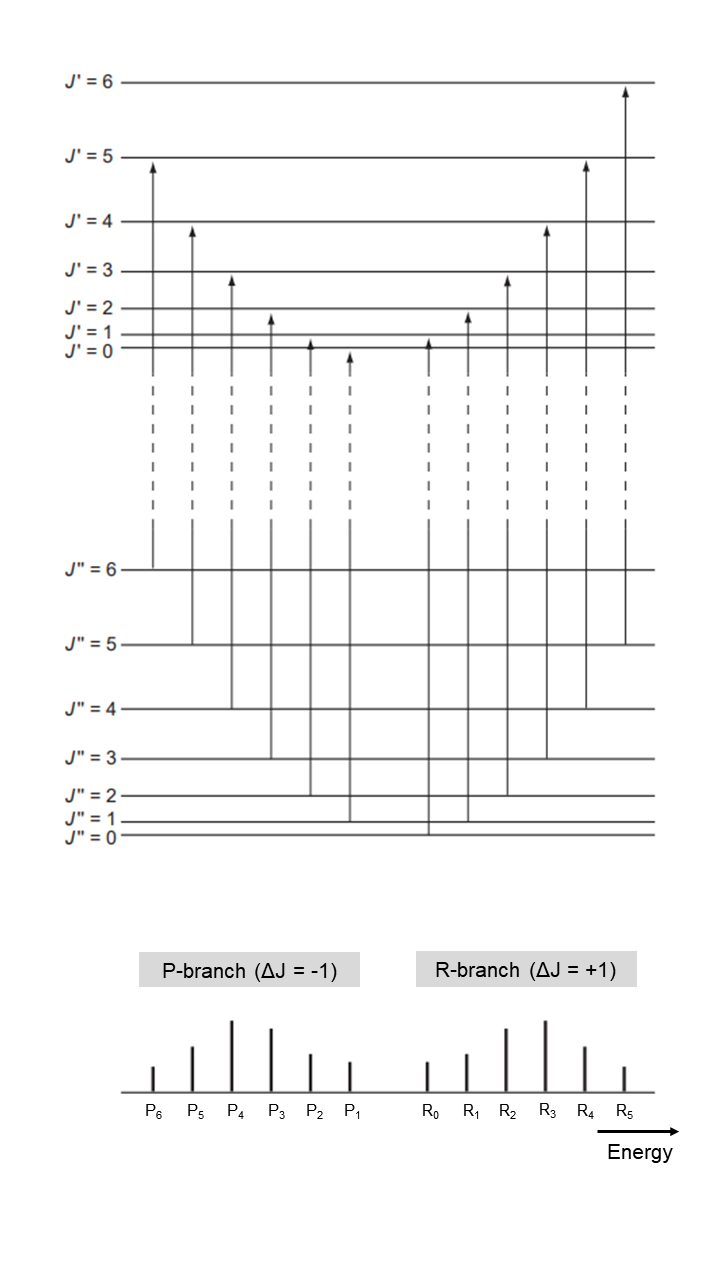
\includegraphics[width=7cm]{irspec}
	\centering
	\caption{A schematic IR spectrum}
	\label{fig:irspec}
\end{figure}
The vibrational state must possess an anisotropic dipole moment wrt. the normal coordinate. \Cref{irsymm} tells us whether a mode is IR-active.
\subsubsection{Raman spectroscopy}

Although complementary to IR spectroscopy, the theory of Raman spectroscopy is fundamentally different. 
An intense beam of laser at an appropriate, non-sweeping, monochromatic freqency is incident upon the sample, and the detector is placed at right angles to the incident beam to collect the scattered photons (note that no overall absorption of photons take place). The scattering can take place in three ways, we report $\Delta\nu$ and $\Delta J$ as ${\Delta\nu,\Delta J}$:
\begin{enumerate}
	\item \textbf{Rayleigh scattering}: Elastic scattering, no change in frequency of the photon, this corresponds to unchanged rot-vibrational level and hence ${0,0}$.
	\item \textbf{Stokes Raman scattering}: Inelastic scattering, reduced energy, corresponds to net excitation of rot-vibrational level, ${0,+2}$ or $+1,\pm2$.
	\item \textbf{Anti-Stokes Raman scattering}: Inelastic scattering, increased energy, corresponds to net relaxation, ${0,-2}$ or ${-1,\pm2}$.
\end{enumerate}
The $\Delta\nu=0$ corresponds to \emph{pure rotational Raman spectroscopy}, it uses low laser frequencies which do not have enough energy to excite the molecule to the next vibrational level, the $\Delta J=\pm2$ correspond to the Stokes and anti-Stokes branches, with the anti-Stokes branch having the same intensities as many rotational levels are thermally accessible at room temperature, so it does not matter whether the intial state is lower or higher. A schematic pure Rotational Raman spectrum is shown in \cref{fig:purerotspec} (the virtual levels are not shown)\footnote{As the branch lettering is $J_{\mathrm{upper}}-J_{\mathrm{lower}} $, both branches are technically $S$ in pure rotational Raman spectra.}:
\begin{figure}[H]
	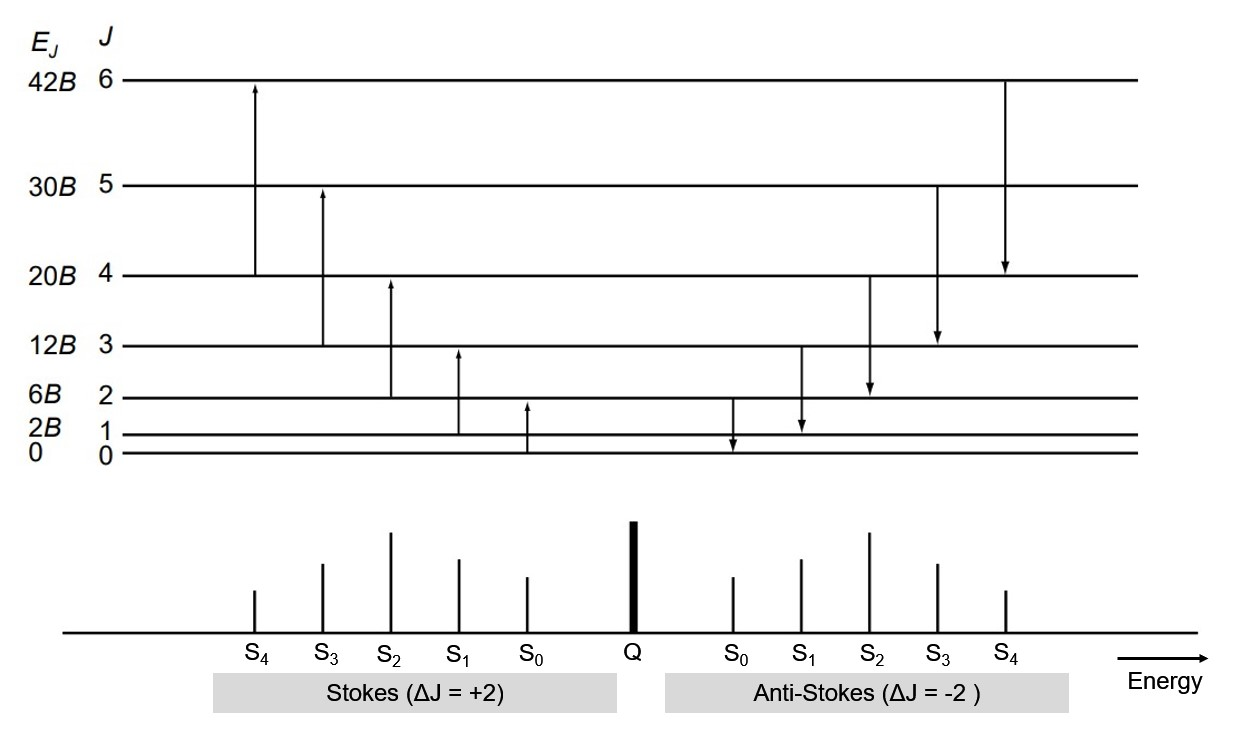
\includegraphics[width=12cm]{ramanspec}
	\centering
	\caption{A schematic pure rotational Raman spectrum}
	\label{fig:purerotspec}
\end{figure}
The $\Delta\nu=\pm1$ corresponds to \emph{vibrational Raman spectroscopy}, which uses high laser frequencies that are enough to excite the molecules vibrationally. The $\Delta\nu=+1$ is the Stokes branch and $\Delta\nu=-1$ is the anti-Stokes. The $\Delta J=\pm2$ should produce $O$- and $S$-branches as rotational fine structures but are too weak to observe in practice. A schematic vibrational Raman spectrum is shown in \cref{fig:vibraman}:
\begin{figure}[H]
	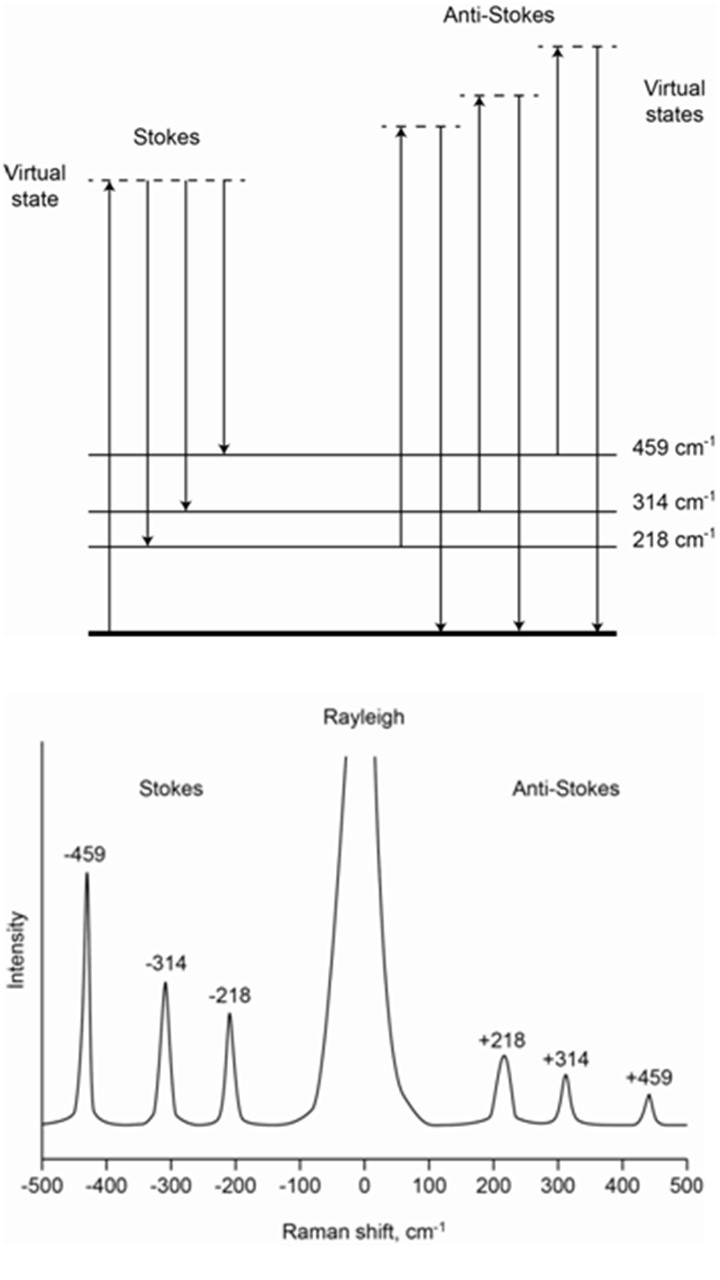
\includegraphics[width=8cm]{vibraman}
	\centering
	\caption{A schematic vibrational Raman spectrum}
	\label{fig:vibraman}
\end{figure}
Whether a vibrational mode is active in vibrational Raman spectroscopy is given by \Cref{irsymm} \hl{not written yet, update with thrm for Raman}.
\subsection{Transition frequencies}

\subsubsection{The vibrating rotor}
The vibrational spectral line spacings are derived from the Morse potential, with energy levels
\begin{equation}
	\ep_v=(v+\tfrac{1}{2} )\widetilde{\omega}-(v+\tfrac{1}{2} )^2\widetilde{\omega}x_e
\end{equation}
The depth of the well, $D_e$, can be found by finding $v_{\mathrm{max}} $, \ie setting $\diff{\ep_v}/{v}=0$:
\begin{equation}
\begin{aligned}
	D_e&=\ep_{\mathrm{max}}-\ep_{\mathrm{ZPE}}\\
&=\frac{\widetilde{\omega}}{4x_e}=\frac{\hbar\omega}{4x_e}
\end{aligned}
\end{equation}
The bond dissociation energy can be found by taking the difference of the well depth and ground state energy:
\begin{equation}
	\ep_B=\widetilde{D}_e-\ep_0=\widetilde{D}_e(1-x_e)^2
\end{equation}
The selection rule for the harmonic oscillator, $\Delta v=\pm 1$, proven in \cref{harmsele}, no longer hold true for the Morse oscillator, where we have $\Delta v=\pm1,\pm2\dots$. However usually only the $0\rightarrow1$ (fundamental), $0\rightarrow2$ (first overtone) are strong and, with the temperature-dependent\footnote{The other bands are not temperature dependent because they all only involve transitions from the ground state which is always thermally accessible.} $1\rightarrow2$ (hot band) and the $0\rightarrow3$ (second overtone) very weak.\par
The transtion frequencies are easy to calculate, some are listed here
\begin{center}
	\begin{tabular}{c|cccc}
	Transition & $0\rightarrow1$ & $0\rightarrow2$ & $0\rightarrow3$ & $1\rightarrow2$\\
	\hline
	$\Delta\ep$&$\widetilde{\omega}-2\widetilde{\omega}x_e $&$2\widetilde{\omega}-6\widetilde{\omega}x_e $&$3\widetilde{\omega}-12\widetilde{\omega}x_e $&$\widetilde{\omega}-4\widetilde{\omega}x_e $
	\end{tabular}
\end{center}
Because the vibrational wavefunction $\psi_n(x\equiv r-r_e)$ and the rotational 
wavefunction $Y^m_J(\theta,\phi)$ have different dependence, \ie degree of 
freedom. Therefore they are independent and we can write (we now adapt the notation in \Cref{vibindex})
\begin{equation}
\begin{aligned}
H\psi_{\mathrm{rot-vib}}&\equiv(H_{\mathrm{rot}}+H_{\mathrm{vib}})Y^m_J\psi_v\\
&=(E_J+E_v)Y^m_J\psi_v\\
&=\lf[BJ(J+1)+\hbar\omega\lf(v+\frac{1}{2}\rt)\rt]\psi_{\mathrm{rot-vib}}
\end{aligned}
\end{equation}
The convention is to write the energies in units of wavenumbers:
\begin{equation}
\widetilde{E}_{v,J}=\widetilde{B}J(J+1)+\widetilde{v}\lf(v+\frac{1}{2}\rt), 
\end{equation}
where 
\begin{equation}
\widetilde{B}=\frac{\hbar}{4\pi\widetilde{c}I},\ \widetilde{v}=\frac{1}{2\pi \widetilde{c}}\sqrt{\frac{k}{\mu}}.
\end{equation}
\begin{equation}
\begin{aligned}
&\Delta v=\pm1\ \text{(overtones allowed but weak)};\\
&\Delta J=\pm1.
\end{aligned}
\end{equation}
We have derived the vibrational spectral frequencies and the rotational frequencies as fine structures around the central vibrational freqencies. There's one problem we need to address, which is that the rotational constant $\widetilde{B}$ is not the same for each vibrational level because $\lgl r \rgl $ increases as vibrational states increases\footnote{This is evident if we examine the functional form of the Morse potential - the oscillator spends more time on the right than the left as the vibrational states are ascended.}. We need to account for that in our derivation for exact frequencies in the rotational fine structure below: 
\begin{equation}
\begin{aligned}
\widetilde{R}_{J''}&=\widetilde{E}_{v=1,J'=J''+1}-\widetilde{E}_{v=0,J''}\\
&=\lf(v+\frac{3}{2} \rt)\tilde{v}+\widetilde{B}_1(J''+1)(J''+2)-\lf(v+\frac{1}{2} \rt)\tilde{v}-\widetilde{B}_0J''(J''+1)\\
&=\tilde{v}_0+(\widetilde{B}_1-\widetilde{B}_0)J''^2+(3\widetilde{B}_1-\widetilde{B}_0)J''+2\widetilde{B}_1 ,\ J''=0,1,2,\cdots. 
\end{aligned}
\end{equation}
Likewise, the $P$-branch has 
\begin{equation}
\widetilde{P}_{J''}=\tilde{v}+(\widetilde{B}_1-\widetilde{B}_0)J''^2-(\widetilde{B}_1+\widetilde{B}_0)J'',\ J''=1,2,3,\cdots, 
\end{equation}
where $J''$ cannot be zero as this implies $J'$ starts at $-1$.\par
In the approximation that $\widetilde{B}_1=\widetilde{B}_0\equiv\widetilde{B}$, we arrive at 
\begin{equation}
\begin{aligned}
&\widetilde{R}_{J''}=\tilde{v}_0+2\widetilde{B}(J''+1)\\
&\widetilde{P}_{J''}=\tilde{v}_0-2\widetilde{B}J''.
\end{aligned}
\end{equation}
\begin{prt}[P and R branch peaks]
\begin{equation}
\begin{aligned}
&(\Delta J=+1)\ \widetilde{R}_{J}=\tilde{v}_0+2\widetilde{B}_1+(3\widetilde{B}_1-\widetilde{B}_0)J+(\widetilde{B}_1-\widetilde{B}_0)J^2 ,\ J=0,1,2,\cdots\\
&(\Delta J=-1)\ \widetilde{P}_{J}=\tilde{v}_0-(\widetilde{B}_1+\widetilde{B}_0)J+(\widetilde{B}_1-\widetilde{B}_0)J^2,\ J=1,2,3,\cdots
\end{aligned}
\end{equation}
\end{prt}
Now, the equilibrium bond length increases as we go up in $v$ with the Morse potential so 
$I$ goes up and $\widetilde{B}$ goes down, so the term $(\widetilde{B}_1-\widetilde{B}_0)J''^2$, although small, 
is always negative and increasingly so with increasing $J''$. 
This means the $P$ branch will be `streched' and the $R$ branch will be `compressed' more and more 
away from the central frequency. 
\subsubsection{Determination of rotational constants}
The general expression for any $J$-transition from $v=0$ to $v=1$ is 
\begin{equation}
\Delta\epsilon=\widetilde{v}_0+\widetilde{B}_1J'(J'+1)-\widetilde{B}_0J''(J''+1).
\end{equation}
Considering peaks originating from the same $J''$ (lower $J$), this gives rise to two peaks, one in the 
$P$ branch and one in the $R$ branch, both labelled with the same $J$ 
(conventionally labelled with lower $J$), and the difference is
\begin{equation}
\widetilde{R}_J-\widetilde{P}_J=2\widetilde{B}_1(2J+1).
\end{equation}
Similarly, for the same $J'$, we can find $\widetilde{B}_0$:
\begin{equation}
\widetilde{R}_{J-1}-\widetilde{P}_{J+1}=2\widetilde{B}_0(2J+1)
\end{equation}
\begin{prt}[Determination of rotational constants]
\begin{equation}
\begin{aligned}
&\widetilde{R}_J-\widetilde{P}_J=2\widetilde{B}_1(2J+1)\\
&\widetilde{R}_{J-1}-\widetilde{P}_{J+1}=2\widetilde{B}_0(2J+1)
\end{aligned}
\end{equation}
\end{prt}
Generally it is assumed that
\begin{equation}
\widetilde{B}_v=\widetilde{B}_e-\widetilde{\alpha}\lf(v+\frac{1}{2} \rt),
\end{equation}
where we need two $\widetilde{B}$'s to determine the equilibrium rotational constant of a hypothetical vibrationless molecule. This can then be used to determine the true equilibrium bond length. 
\subsubsection{Q-branch}
The selection rule $\Delta J=\pm1$ for IR spectroscopy holds true strictly for \emph{parallel vibrations} of linear molecules only, for molecules that have a perpendicular component of angular momentum, $\Delta J=0$ is possible\footnote{$J$ is \emph{defined} as the angular momentum in the direction of the principal axis, note this is the intrinsic axis instead of the laborartory $z$-axis which defines $m$.}. Examples include

\begin{itemize}
	\item Any non-linear molecule, as there are other axes of rotation other than the principal axis, the angular momentum about which $J$ is defined.
	\item Linear triatomic molecules, which have two degenerate bending modes, which create an oscillating dipole perpendicular to the principal axis, can combine to give rotational motions about the principal axis. This is the \textit{vibrational angular momentum}. 
	\item Diatomics with electronic orbital angular momentum, like NO, whose ground state term symbol is $^2\Pi$, this angular momentum is intrinsic in origin, rather than induced by vibration
\end{itemize}
Since all quantum mechanical angular momenta are quantised in the same way (in steps of $\hbar$), a photon can excite these angular momenta. This means that conservation of angular momentum is now possible without 
a change in $J$, 
\begin{prt}[Selection rules for perpendicular vibrations]
\begin{equation}
\begin{aligned}
&\Delta J=0,\ \pm1\\
&\Delta v=\pm1,\ \pm2,\ \cdots
\end{aligned}
\end{equation}
\end{prt}
The $Q$-branch consists of all transitions with the same $J$, and the frequencies are given by 
\begin{equation}
\begin{aligned}
\epsilon'-\epsilon''=&\lf[\lf(1+\frac{1}{2}\rt)\widetilde{\omega}-\lf(1+\frac{1}{2}\rt)^2\widetilde{\omega}x_e +\widetilde{B}_1J(J+1) \rt]-\\
&\lf[\lf(0+\frac{1}{2}\rt)\widetilde{\omega}-\lf(0+\frac{1}{2}\rt)^2\widetilde{\omega}x_e +\widetilde{B}_0J(J+1)\rt]\\
=&\widetilde{\omega}-2\widetilde{\omega}x_e+(\widetilde{B}_1-\widetilde{B}_0)J(J+1)\\
\equiv&\widetilde{\omega}_0+(\widetilde{B}_1-\widetilde{B}_0)J(J+1).
\end{aligned}
\end{equation}
\begin{prt}[$Q$-branch peaks]
$Q$-branch peaks occur at
\begin{equation}
\widetilde{\omega}_0+(\widetilde{B}_1-\widetilde{B}_0)J(J+1).
\end{equation}
\end{prt}
As $(\widetilde{B}_1-\widetilde{B}_0)$ is small, and \emph{positive} in this case as bending will result in smaller moment of inertia, this results in the spreading (towards higher wavenumbers) out of the Q-branch. This has effects on the $P$- and $R$-branches as well: now $R$ branch will be spread out away from the central freqency and $P$ will be compressed away from the central freqency, opposite of that in parallel strectches. All this is shown in \cref{fig:qbranch}
\begin{figure}[H]
	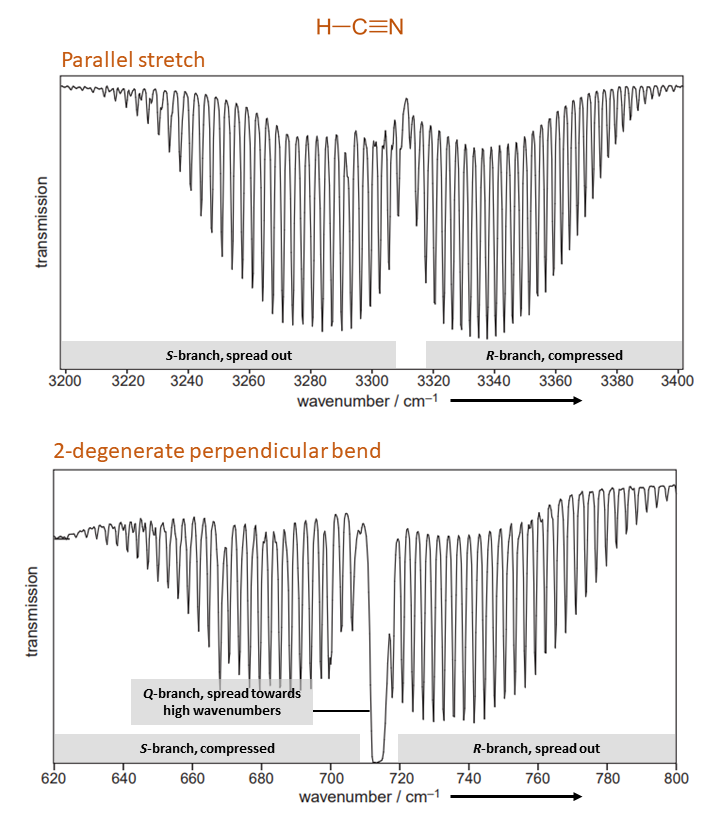
\includegraphics[width=12cm]{qbranch}
	\centering
	\caption{The IR spectrum of HCN, showing $Q$ branch in only one of the vibrational modes.}
	\label{fig:qbranch}
\end{figure}
The presence of $Q$-branch can be a diagnostic
\begin{prt}[Presence of $Q$-branch]
The absence of $Q$-branch in any of the vibrational modes proves that the molecule has to be linear.
\end{prt}
\subsection{Polyatomic molecules}
\label{polyvib}
\subsubsection{Normal coordinates}
\begin{thrm}[Normal coordinates]
\label{sym_of_vibfun}
In any molecular vibration mode $i$ it is always possible to define a normal coordinate $Q_i$ that can replace the scaled coordinate $q$ in the vibrational wavefunction.
\end{thrm}
\begin{proof}
	The problem with polyatmoic molecules is that they have $3N-5$ (linear) or $3N-6$ (non-linear) normal modes, therefore the same number of vibrational coordinates, $q_i$, and we can write the change in potential energy as
\begin{equation}
\begin{aligned}
	\dif V&=\frac{1}{2}\sum_{i=1}^{N_{\mathrm{vib}}}\sum_{j=1}^{N_{\mathrm{vib}}}\diffp{V}{q_i,q_j}q_iq_j+(\text{higher derivatives})\\
	&=\frac{1}{2}\sum_{i=1}^{N_{\mathrm{vib}}}\sum_{j=1}^{N_{\mathrm{vib}}}f_{ij}q_iq_j+\dots
\end{aligned}
\end{equation}
Unfortunately, the cross-terms makes the \sch intractable. A theorem from classical mechanics can transform the cross terms into \emph{normal coordinates}:
\begin{equation}
	\dif V\approx\frac{1}{2}\sum_{j=1}^{N_{\mathrm{vib}}}F_jQ_j^2
\end{equation}
\end{proof}
\begin{prt}[Symmetry of normal coordinates]
The normal coordinate $Q_i$ has the same symmetry as the normal mode.
\end{prt}
\begin{proof}
	The normal coordinate $Q_i$ \emph{defines} the normal mode as the linear combination of vibrational coordinates that make up the normal mode. Therefore \emph{must} transform as the symmetry species of the normal mode. This pointing out the chicken-and-egg situation rather than a proof.
\end{proof}
\subsubsection{Symmetry of vibrational wavefunctions}
As the transition probability involves evaluating integrals of the form $\lgl \psi_i |\bvec{\mu}|\psi_j  \rgl $, we need to work out the symmetry species spanned by the vibrational wavefunctions. 
\begin{thrm}[Symmetry of vibrational wavefunctions]
For harmonic oscillators, odd state vibrational wavefunctions always transform as the totally symmetric IR.\par
Even state vibrational wavefunctions always transform as the IR of the normal mode.\par
For degenerate normal modes, the first excited state transforms as the normal mode, but higher excited states are more complex \hl{what?}
\end{thrm}
\begin{proof}
	As the unnormalised ground state is
	\begin{equation}
		\psi_0=e^{-\frac{1}{2}Q_i^2}
	\end{equation}
	For a non-degenerate irrep, this must return characters as 1's, \ie the totally symmetric IR.\par
	The first excited state is
	\begin{equation}
		\psi_1=Q_ie^{-\frac{1}{2}Q_i^2},
	\end{equation}
	we know the exponential bit transforms as the tot. sym. IR, and that $Q_i$ transforms as the normal mode (\Cref{sym_of_vibfun}), therefore $\psi_1$ transforms as the symmetry species of the normal mode. \par
	The form of the Hermite polynomials \hl{is this true? specific only to Hermite?} dictates that even-numbered functions contains only even exponents and constants, and that odd-numbered functions contains only odd exponents and no constants, \ie factorisable to $[Q_i(\text{tot. sym. function})]$, which means they all transform as the normal mode. 
\end{proof}
\subsubsection{Symmetry selection rules for infrared}
For transition between energy levels of a single normal mode, we assume we start at the ground state, we need to know whether the integral
\begin{equation}
R_{v_i,v_i'}=\lgl\psi_{v_i'}|\mu|\psi_{v_i} \rgl
\end{equation}
is non-zero, where $\mu$ transforms like the principle Cartesian axes:
\begin{defi}[Dipole moment operator]
As the dipole moment $\bvec{\mu}$ is only dependent on the normal coordinate $\bvec{Q_i}$, we can write
\begin{equation}
\bvec{\mu}=\bvec{\mu}_0+\lf(\diff{\bvec{\mu}}{Q_i}\rt)_{Q_i=0} Q_i+\frac{1}{2}\lf(\diff[2]{\bvec{\mu}}{Q_i} \rt)_{Q_i=0}Q_i^2+\dots
\end{equation}
If we make the approximation that the partial charges are constant \ie dipole moment varies linearly with normal coordinate, with the first term vanished by orthonormality, we are left with the definition of the dipole moment:
\begin{equation}
\bvec{\mu}\equiv \lf(\diff{\bvec{\mu}}{x}\rt)_0 Q_i
\end{equation}
\end{defi}
Invoking theorem \hl{which one}, we arrive at the result
\begin{thrm}[Transition rules]
\label{irsymm}
For a fundamental transition (transitions from the ground state energy of a normal mode to an excited state of the same mode) to be allowed in infrared, the IR of the normal mode has to be the same as that of x, y or z.
\end{thrm}
However symmetry allowed transitions can still have their integrals evaluated to zero by functional forms determined not by symmetry. For example, the selection rule for the harmonic oscillator is $\nu=\pm 1$, this is derived from the ladder operators:\par
As stated above, we can always write the normal coordinate as 
\begin{equation}
Q_i=\lf(\frac{\hbar}{2\mu\omega} \rt)^{1/2}(a_-+a_+)
\end{equation}
where the ladder operators also have their scaled coordinate replaced by the normal coordinate. It is now easy to write
\begin{equation}
\label{harmsele}
\begin{aligned}
\lgl v_i|\bvec{\mu}|v_j\rgl&\propto \lgl v_i|(a_-+a_+)|v_j \rgl\\
&=\delta_{i,j-1}+\delta_{i,j+1}
\end{aligned}
\end{equation}
and it is apparent that only when $j=i\pm 1$, the matrix element is nonzero. 
\subsection{Electronic spectroscopy}

\subsubsection{The Franck-Condon principle}
The Einstein B coefficient for induced absorption or emission\footnote{The A coefficient is for spontaneous emission.} is given as 
\begin{equation}
\label{einsteincoeff}
	B_{mn}=\frac{1}{3\ep_0\hbar^2}|\lgl \psi_m |\uvec{\mu}|\psi_n  \rgl|^2
\end{equation}
Under the Born-Oppenheimer approximation, ignoring the rotational changes, as they are too fine to be resolved, we can write
\begin{equation}
	\psi_i=\psi_{i,E}\psi_{i,V},\ \uvec{\mu}=\uvec{\mu}_E+\uvec{\mu}_V
\end{equation}
The transition dipole moment is now
\begin{equation}
\begin{aligned}
	&|\lgl \psi'' |\uvec{\mu}|\psi'  \rgl|^2\\
	=&|\lgl \psi''_E\psi''_V|\uvec{\mu}_E+\uvec{\mu}_V |\psi_E'\psi_V'  \rgl |^2\\
	=&|\lgl \psi''_E\psi''_V|\uvec{\mu}_E|\psi_E'\psi_V'  \rgl+\lgl \psi''_E\psi''_V|\uvec{\mu}_V|\psi_E'\psi_V'  \rgl |^2\\
	=&|\lgl \psi''_E|\uvec{\mu}_E|\psi_E'  \rgl \lgl \psi''_V | \psi_V' \rgl+ \lgl \psi''_E | \psi_E' \rgl \lgl \psi''_V|\uvec{\mu}_V|\psi_V'  \rgl |^2\\
	=&|\lgl \psi''_E|\uvec{\mu}_E|\psi_E'  \rgl|^2 |\lgl \psi''_V | \psi_V' \rgl|^2
\end{aligned}
\end{equation}
The electronic wavefunctions are orthonormal, but not the vibrational states \emph{belonging to different electronic states} as they are on different Morse potentials and are solutions to different Schro\"dinger equations.\par
The first bit is the electronic transition dipole, and group theory can tell us whether that vanishes. The second part is known as the \emph{Franck-Condon factor}, which tells us the extent of overlap between two vibrational wavefunctions. The \emph{Franck-Condon principle} is the assumption that there's no change in bond length before and after the electronic transition \ie the overlap F-C factor can tell us the probability of transition.
\begin{thrm}[The Franck-Codon principle]
Because the nuclei are much more massive than electrons, an \emph{electronic} transition takes place while the nuclei in a molecule are effectively stationary. The transition probability between two vibrational states in two electronic states is given by $|\lgl \psi''_V | \psi_V' \rgl|^2$.
\end{thrm}
This will give progressions that start from the lower vibrational states $v''=0,1,2,\dots$, which each successive progression at lower wavenumbers and lower intensities as the states become less populated.\par
The transition energies can be represented as follows
\begin{equation}
\begin{aligned}
	\widetilde{v}'-\widetilde{v}''&=(\ep_0'-\ep_0'')+\{[(v'+\tfrac{1}{2})\widetilde{\omega}'_e-\widetilde{\omega}'_ex_e'(v'+\tfrac{1}{2} )^2]-[(v''+\tfrac{1}{2})\widetilde{\omega}''_e-\widetilde{\omega}''_ex_e''(v''+\tfrac{1}{2} )^2]\}\\
	&\equiv T_e+\Delta \widetilde{E}_v 
\end{aligned}
\end{equation}
This allows us to compute parameters such as the equilibrium bond length and the dissociation energy of an excited electronic mode.
